% !TEX root = ../thesis.tex

\chapter{Syntetická časť}
\label{methodology}
V tejto časti si prejdeme konceptuálny návrh riešenia na predikciu víťazného tímu v profesionálnych esport zápasoch v hre League of Legends a bližšie sa pozrieme na metódy a hodnoty, ktoré budú potrebné pri jednotlivých fázach z návrhu riešenia, a na finálnu tvorbu prototypu. 
\section{Konceptuálny návrh riešenia}

 \begin{figure}[ht!]
	
	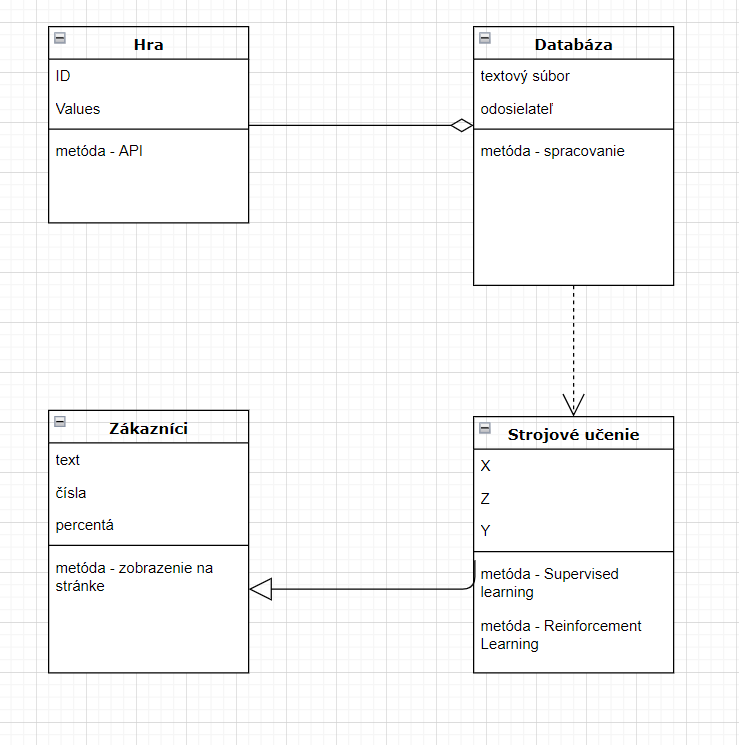
\includegraphics[width=.9\textwidth]{figures/navrhriesenia}
	\centering
	\caption{ Konceptuálny návrh riešenia \label{koncept}}
	
\end{figure}

Ako môžeme vidieť na obrázku \ref{koncept}, na návrh riešenia treba spracovať 4 fázy : 

\begin{enumerate}
	\item Prevziať potrebné dáta z hier cez databázy
	\item Spracovať ich do čitateľnej verzie pre umelú inteligenciu
	\item Použiť dáta na natrénovanie modelu
	\item Spracovať výsledky do čitateľnej formy pre zákazníkov
\end{enumerate}

\section{Prevzatie dát z databáz}
V databázach bolo nie len veľké množstvo druhov dát, ale aj spôsobov akým tieto dáta získať. Bola možnosť zobrať buď dáta zo všetkých hier, čiže aj neprofesionálnych alebo čisto hry iba z profesionálnych turnajov. Po dlhom uvažovaní a viacerých skúškach sme sa rozhodli použiť dáta iba z hier profesionálnych turnajov z celého sveta a konkrétne z posledných 5 mesiacov. Dokopy je rôznych inštancií, ktoré berieme do úvahy viac ako 250 000.

\subsection{Finálny druh dát}
Používané dáta budú 4 druhov. Meno šampióna, pozícia v hre, počet hier, miera výhry. Tieto dáta budú v 2 inštanciach relácií a to v relácií pozorovaný šampión vo vzťahu s jeho tímom a druhej vo vzťahu s nepriateľským tímom.

\subsection{Úprava dát}
Kedže databázy nie sú predpripravené na instantné využitie pri umelej inteligencii, tak sme dáta museli prispôsobiť do podoby, ktoré python, konkrétne scikit learn vie načítať. Dát je príliš veľa na ručnú úpravu, preto sme napísali krátky kód v jave, ktorý načíta databázy, každé slovo dá do uvozdoviek, dá medzi ne čiarku a odstráni všetky tabulátory a medzery.

\subsection{Tokenizácia dát}
Vzhľadom na veľké množstvo rôznych šampiónov, sme sa rozhodli ich rozdeliť na určité kategórie podľa ich významu v hre a ich pozícii v tíme.
V hre je 5 pozícií a pre káždú sme vybrali najčastejšie kategórie, do ktorých patria šampióni. Tu sú kategória aj s krátkymi popismi :
\begin{enumerate}
	\item TOP - pozícia na vrchu mapy, väčšinou izolovaná, až do neskorších fáz hry
	 \begin{itemize}
		\item laner - šampión, ktorý si zakladá na ich sile v prvých štádiách hry
		\item splitpusher - šampión, ktorý je rád izolovaný a rýchlo ničí veže
		\item teamfightdamage - šampión, ktorý exceluje v neskorších fázach hry a jeho primárnou priotiou je urobiť čo najväčšie poškodenie nepriateľským šampiónom počas tímového boja
		\item teamfightcc - skratka cc znamená crowd control, myslené ako udržanie nepriateľského šampióna v nehybnom stave, zatiaľ čo ho spoluhráči zabijú
	\end{itemize}
	\item JUNGLE - pozícia, ktorá sa voľne pohybuje po celej mape, zabíja jeho campy(6 rozdelených miest, kde zabíja monštrá za peniaze a obnovia sa dookola za 2 a pol až 5 minút)  a aplikuje "ganky" (kalkulované útoky na časť mapy)
	\begin{itemize}
		\item clearer - jungler(šampión v jungli), ktorý si zakladá na ich rýchlosti zabíjaní campov
		\item ganker - jungler, ktorého hlavnou úlohou je čo najrýchlejšie pripraviť a vykonať, čo najvyšší počet gankov
		\item early - jungler, ktorý je najsilnejší v prvých častiach hry
		\item late - jungler, ktorý sa snaží nezomierať a pretrpieť do neskorších fáz hry, v ktorých je najsilnejší
		\item teamfightdamage - jungler, ktorý si v neskorších fázach hry zakladá na výške poškodenia počas tímového boja
		\item teamfightcc - jungler, ktorý si v neskorších fázach hry zakladá na možnosti znehybniť jedného alebo viacerých nepriateľských šampiónov
	\end{itemize}
	\item MID - centrovaná pozícia, blízko ku TOPu a aj BOTu. Význám sa odvíja od plánu ostatných spoluhráčov
	\begin{itemize}
		\item scaler - šampión, ktorý sa snaží udržať hru v rovnovážnom stave, lebo čím je dlhšia hra tým je silnejší
		\item roamer - šampión, ktorý sa rád pohybuje po mape a pomáha ostatným spoluhráčom
		\item teamfightdamage 
		\item teamfightcc 
	\end{itemize}
	\item BOT - duálna pozícia s pozíciou SUP na spodku mapy. Priorita je poskytnutie poškodenia z bezpečnej vzdialenosti
	\begin{itemize}
		\item poker - adc(šampión v pozícii BOT), ktoré sa nerád zapája do intenzívneho súboja, ale z veľkej diaľky ostreluje nepriateľov
		\item fighter - adc, ktorý rado dostane do blízkosti jedného alebo viacerých nepriateľov a snaží sa urobiť čo najväčšie poškodenie aj keby malo zomrieť 
		\item utility - adc, ktorého prioritou nie je vysoké poškodenie, ale poskytovanie obnovy života alebo štítov spoluhráčom a zároveň spomľovanie alebo odhalenie nepriateľov
		\item fronttoback - adc, ktoré je najlepšie v situáciach, kde nepriateľský tím bojuje s jeho tímom a ono sa rýchlo pohybuje dnu a von z boja
	\end{itemize}
\item SUP - pomocná pozícia, ktorá slúži na zosilnenie a ochranu spoluhráčov
\begin{itemize}
	\item engage - support(šampión v pozícii SUP), ktorého prioritou je odchytiť nepriateľského šampióna a tým nepriamo začať tímovy súboj
	\item peel - support, ktorého priorita je ochrániť spoluhráčov tým, že znehybnia nepriateľov, aby spoluhráči mohli bezpečne dávať poškodenia nepriateľskému tímu
	\item enchanter - support, ktorý poskytuje spoluhráčom uzdravenia a štíty, poprípade znovuzrodenie
\end{itemize}
\end{enumerate}
\section{Opis metód}
Hlavné metódy pri učení nášho modelu.
\subsection{Supervised learning}
Podkategória umelej inteligencie, ktorá používa daný dataset na natrénovanie modelu.

\subsection{Reinforcement learning}
Časť umelej inteligencie, pri ktorej sa sledujú kroky inteligentných agentov na maximalizáciu efektívnosti dosiahnutia cieľa.
